\chapter{Related work}
\section{Boundary attack}
\gls{ba} \cite{boundary_attack} is a decision-based adversarial attack. The basic intuition of \gls{ba} differs from traditional adversarial attacks. Unlike these traditional adversarial attacks, where the original image is moved through search space in order to become adversarial, \gls{ba} starts from an input that is already adversarial. This input is then moved closer to the original image, while staying adversarial.\\

The attack has to be initialized with an already adversarial input. Two different approaches can be taken depending on the attack setting. In the untargeted case, the input can be sampled from a maximum entropy distribution given the valid domain of this input. Samples that are not adversarial are rejected. In the case of a targeted attack, the input is a sample from the dataset that is classified as the target class by the model under attack.\\

\gls{ba} iteratively updates the adversarial image by performing a step orthogonal to the original image and a step towards this image. In iteration $k$, a perturbation $\eta_k$ is sampled from a Gaussian distribution. This perturbation is rescaled and added to the adversarial image. From this new position in search space, the step towards the original image is taken. This way the path of the attack follows the decision boundary, hence the name of the attack. The intuition of the \gls{ba} is shown in Figure~\ref{fig:boundary_attack_intuition}. The attack can only follow the boundary if the adversarial image is already near the boundary. The starting image is projected onto the boundary using binary search to ensure that the adversarial image is in the vicinity of the boundary.\\

The step sizes are adjusted according to local geometry of the boundary. The orthogonal step size $\delta$ is adjusted so that approximately half of the orthogonal perturbations is still adversarial. This approach is based on trust region methods \cite{trm}. The step size towards the original image $\epsilon$ is adjusted using the same principle, but here a user specified threshold is used. The decision boundary tends to become flatter, the closer to the original image the attack gets. Therefore the algorithm converges when $\epsilon$ converges to zero.\\

\gls{bba} \cite{brunner_guessing_2019} improves the original \gls{ba} in three different ways. The first improvement is a biased sampling technique. The key idea behind this that most previous attacks yield adversarial examples with high frequencies in the image. By sampling the perturbations in the first step of the \gls{ba} from a low frequency distribution, the frequency of the created adversarial example will be lowered as well. \gls{bba} does this by sampling from a Perlin noise \cite{perlin} distribution.\\

\begin{figure}
\centering
\tikzset{every picture/.style={line width=0.75pt}} %set default line width to 0.75pt        
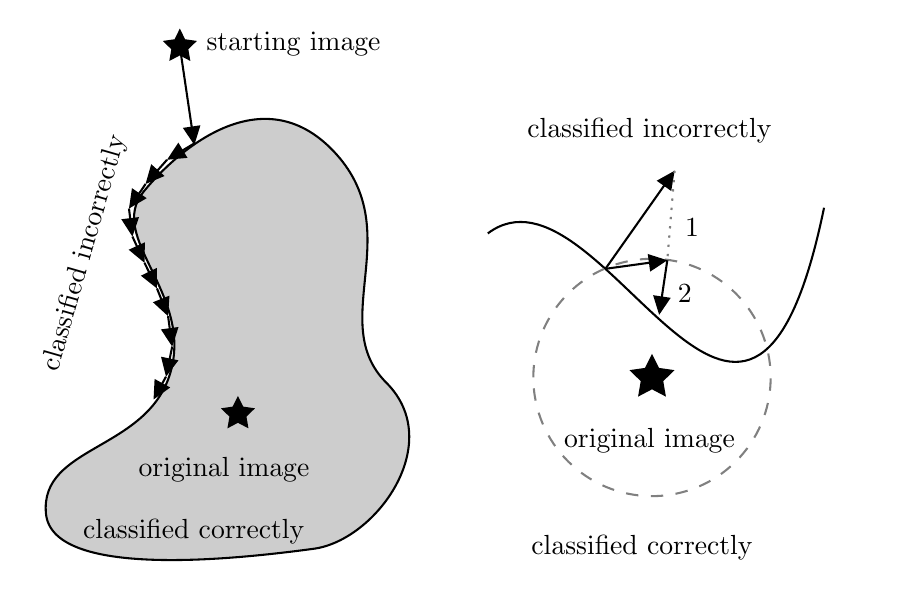
\begin{tikzpicture}[x=0.75pt,y=0.75pt,yscale=-1,xscale=1]
%uncomment if require: \path (0,300); %set diagram left start at 0, and has height of 300

%Shape: Polygon Curved [id:ds5185908380685693] 
\draw  [fill={rgb, 255:red, 155; green, 155; blue, 155 }  ,fill opacity=0.5 ] (77.12,91.56) .. controls (95.12,69.56) and (136.12,35.56) .. (170.12,73.56) .. controls (204.12,111.56) and (165.12,154.56) .. (194.12,183.56) .. controls (223.12,212.56) and (189.12,259.56) .. (159.12,263.56) .. controls (129.12,267.56) and (33.12,279.56) .. (30.12,246.56) .. controls (27.12,213.56) and (79.12,216.56) .. (90.12,178.56) .. controls (101.12,140.56) and (59.12,113.56) .. (77.12,91.56) -- cycle ;
%Shape: Star [id:dp7170747564600322] 
\draw  [fill={rgb, 255:red, 0; green, 0; blue, 0 }  ,fill opacity=1 ] (122.62,191.06) -- (124.83,195.53) -- (129.76,196.24) -- (126.19,199.72) -- (127.03,204.63) -- (122.62,202.31) -- (118.22,204.63) -- (119.06,199.72) -- (115.49,196.24) -- (120.42,195.53) -- cycle ;
%Shape: Star [id:dp10477759386916752] 
\draw  [fill={rgb, 255:red, 0; green, 0; blue, 0 }  ,fill opacity=1 ] (94.62,14.06) -- (96.83,18.53) -- (101.76,19.24) -- (98.19,22.72) -- (99.03,27.63) -- (94.62,25.31) -- (90.22,27.63) -- (91.06,22.72) -- (87.49,19.24) -- (92.42,18.53) -- cycle ;
%Straight Lines [id:da2531323347021954] 
\draw    (94.62,21.56) -- (101.19,66.01) ;
\draw [shift={(101.62,68.98)}, rotate = 261.6] [fill={rgb, 255:red, 0; green, 0; blue, 0 }  ][line width=0.08]  [draw opacity=0] (8.93,-4.29) -- (0,0) -- (8.93,4.29) -- cycle    ;
%Straight Lines [id:da6594852147606747] 
\draw    (101.79,68.14) -- (91.03,74.6) ;
\draw [shift={(88.46,76.14)}, rotate = 329.04] [fill={rgb, 255:red, 0; green, 0; blue, 0 }  ][line width=0.08]  [draw opacity=0] (8.93,-4.29) -- (0,0) -- (8.93,4.29) -- cycle    ;
%Straight Lines [id:da6002841525279263] 
\draw    (88.46,76.14) -- (80.11,85.56) ;
\draw [shift={(78.12,87.81)}, rotate = 311.53] [fill={rgb, 255:red, 0; green, 0; blue, 0 }  ][line width=0.08]  [draw opacity=0] (8.93,-4.29) -- (0,0) -- (8.93,4.29) -- cycle    ;
%Straight Lines [id:da9148455444041863] 
\draw    (78.12,87.81) -- (71.8,97.16) ;
\draw [shift={(70.12,99.64)}, rotate = 304.06] [fill={rgb, 255:red, 0; green, 0; blue, 0 }  ][line width=0.08]  [draw opacity=0] (8.93,-4.29) -- (0,0) -- (8.93,4.29) -- cycle    ;
%Straight Lines [id:da47669503735159546] 
\draw    (70.12,99.64) -- (71.42,110.17) ;
\draw [shift={(71.79,113.14)}, rotate = 262.96] [fill={rgb, 255:red, 0; green, 0; blue, 0 }  ][line width=0.08]  [draw opacity=0] (8.93,-4.29) -- (0,0) -- (8.93,4.29) -- cycle    ;
%Straight Lines [id:da26104674623686774] 
\draw    (71.79,113.14) -- (76.37,123.08) ;
\draw [shift={(77.62,125.81)}, rotate = 245.27] [fill={rgb, 255:red, 0; green, 0; blue, 0 }  ][line width=0.08]  [draw opacity=0] (8.93,-4.29) -- (0,0) -- (8.93,4.29) -- cycle    ;
%Straight Lines [id:da9792015265988265] 
\draw    (77.62,125.81) -- (82.31,135.45) ;
\draw [shift={(83.62,138.14)}, rotate = 244.06] [fill={rgb, 255:red, 0; green, 0; blue, 0 }  ][line width=0.08]  [draw opacity=0] (8.93,-4.29) -- (0,0) -- (8.93,4.29) -- cycle    ;
%Straight Lines [id:da8018833944649997] 
\draw    (83.62,138.14) -- (87.84,148.69) ;
\draw [shift={(88.96,151.48)}, rotate = 248.2] [fill={rgb, 255:red, 0; green, 0; blue, 0 }  ][line width=0.08]  [draw opacity=0] (8.93,-4.29) -- (0,0) -- (8.93,4.29) -- cycle    ;
%Straight Lines [id:da7469050329272713] 
\draw    (88.96,151.48) -- (90.55,163.17) ;
\draw [shift={(90.96,166.14)}, rotate = 262.23] [fill={rgb, 255:red, 0; green, 0; blue, 0 }  ][line width=0.08]  [draw opacity=0] (8.93,-4.29) -- (0,0) -- (8.93,4.29) -- cycle    ;
%Straight Lines [id:da36931886382540347] 
\draw    (90.96,166.14) -- (88.57,177.7) ;
\draw [shift={(87.96,180.64)}, rotate = 281.69] [fill={rgb, 255:red, 0; green, 0; blue, 0 }  ][line width=0.08]  [draw opacity=0] (8.93,-4.29) -- (0,0) -- (8.93,4.29) -- cycle    ;
%Straight Lines [id:da3125285737899821] 
\draw    (87.96,180.64) -- (83.39,189.01) ;
\draw [shift={(81.96,191.64)}, rotate = 298.61] [fill={rgb, 255:red, 0; green, 0; blue, 0 }  ][line width=0.08]  [draw opacity=0] (8.93,-4.29) -- (0,0) -- (8.93,4.29) -- cycle    ;

%Curve Lines [id:da7332610230112269] 
\draw    (243,111.62) .. controls (297.92,70.43) and (367.93,279.11) .. (405,99.26) ;
%Shape: Star [id:dp6998768571531213] 
\draw  [fill={rgb, 255:red, 0; green, 0; blue, 0 }  ,fill opacity=1 ] (322.11,170.74) -- (325.14,176.87) -- (331.9,177.85) -- (327.01,182.62) -- (328.16,189.36) -- (322.11,186.18) -- (316.06,189.36) -- (317.22,182.62) -- (312.32,177.85) -- (319.09,176.87) -- cycle ;
%Straight Lines [id:da9467918607674688] 
\draw    (299.68,128.68) -- (331.29,83.87) ;
\draw [shift={(333.02,81.42)}, rotate = 125.2] [fill={rgb, 255:red, 0; green, 0; blue, 0 }  ][line width=0.08]  [draw opacity=0] (8.93,-4.29) -- (0,0) -- (8.93,4.29) -- cycle    ;
%Shape: Ellipse [id:dp07084957668985581] 
\draw  [color={rgb, 255:red, 128; green, 128; blue, 128 }  ,draw opacity=1 ][dash pattern={on 4.5pt off 4.5pt}] (264.94,181.03) .. controls (264.94,149.46) and (290.54,123.86) .. (322.11,123.86) .. controls (353.69,123.86) and (379.28,149.46) .. (379.28,181.03) .. controls (379.28,212.61) and (353.69,238.2) .. (322.11,238.2) .. controls (290.54,238.2) and (264.94,212.61) .. (264.94,181.03) -- cycle ;
%Straight Lines [id:da7547924674466151] 
\draw    (299.68,128.68) -- (326.52,124.97) ;
\draw [shift={(329.49,124.56)}, rotate = 172.13] [fill={rgb, 255:red, 0; green, 0; blue, 0 }  ][line width=0.08]  [draw opacity=0] (8.93,-4.29) -- (0,0) -- (8.93,4.29) -- cycle    ;
%Straight Lines [id:da7777022216727221] 
\draw    (329.49,124.56) -- (326.01,147.88) ;
\draw [shift={(325.57,150.85)}, rotate = 278.49] [fill={rgb, 255:red, 0; green, 0; blue, 0 }  ][line width=0.08]  [draw opacity=0] (8.93,-4.29) -- (0,0) -- (8.93,4.29) -- cycle    ;
%Straight Lines [id:da931484330606797] 
\draw [color={rgb, 255:red, 128; green, 128; blue, 128 }  ,draw opacity=1 ] [dash pattern={on 0.84pt off 2.51pt}]  (333.02,81.42) -- (329.49,124.56) ;


% Text Node
\draw (328.21,263) node   [align=left] {\begin{minipage}[lt]{96.27pt}\setlength\topsep{0pt}
classified correctly
\end{minipage}};
% Text Node
\draw (326.21,62) node   [align=left] {\begin{minipage}[lt]{96.27pt}\setlength\topsep{0pt}
classified incorrectly
\end{minipage}};
% Text Node
\draw (325.12,211.56) node   [align=left] {\begin{minipage}[lt]{68pt}\setlength\topsep{0pt}
original image
\end{minipage}};
% Text Node
\draw (112.21,255.14) node   [align=left] {\begin{minipage}[lt]{96.27pt}\setlength\topsep{0pt}
classified correctly
\end{minipage}};
% Text Node
\draw (106,13) node [anchor=north west][inner sep=0.75pt]   [align=left] {starting image};
% Text Node
\draw (50.21,116) node  [rotate=-286.01] [align=left] {\begin{minipage}[lt]{96.27pt}\setlength\topsep{0pt}
classified incorrectly
\end{minipage}};
% Text Node
\draw (120.12,225.56) node   [align=left] {\begin{minipage}[lt]{68pt}\setlength\topsep{0pt}
original image
\end{minipage}};
% Text Node
\draw (383.43,108.71) node   [align=left] {\begin{minipage}[lt]{68pt}\setlength\topsep{0pt}
1
\end{minipage}};
% Text Node
\draw (379.9,140.85) node   [align=left] {\begin{minipage}[lt]{68pt}\setlength\topsep{0pt}
2
\end{minipage}};


\end{tikzpicture}
\caption[Intuition of the Boundary Attack]{Intuition behind the Boundary Attack. On the left the path of the attack is shown. The first step is a projection onto the boundary, afterwards it follows the decision boundary of the class of the original image. Each arrow represents one iteration of the attack. On the right, the two different steps of each iteration can be seen. In the first step, a random direction is sampled and projected onto a sphere around the original image. A step towards the original image is taken from this new position. Image inspired by \cite{boundary_attack}.}
\label{fig:boundary_attack_intuition}
\end{figure}